\chapter{基因表达：转录与翻译}\label{ch:b1:gene-expression}

一个含三万个\omterm{thm:b1:nucleic-acids:helix}{碱基对}的\omterm{def:b1:genomes:gene}{基因}，在十五分钟内被转录，
复制成一条工作副本，剪短至两千个碱基，
运出\omterm{def:b1:eukaryotic-cell:nucleus}{细胞核}，并由二十五个\omterm{def:b1:gene-expression:ribosome}{核糖体}同时翻译成
一条含五百个\omterm{def:b1:proteins:aminoacid}{氨基酸}的\omterm{def:b1:proteins:peptide}{蛋白质}——每四秒一个，只要副本尚存，
便持续进行。\omterm{def:b1:cell-unit-of-life:cell}{细胞}在这一过程上耗费的能量，
多于其他任何活动。本章追踪信息从 \omterm{def:b1:nucleic-acids:chain}{DNA}
到\omterm{def:b1:proteins:peptide}{蛋白质}的流动：\omterm{def:b1:genomes:gene}{基因}转录为 \omterm{def:b1:nucleic-acids:chain}{RNA}，真核生物中对该 \omterm{def:b1:nucleic-acids:chain}{RNA} 的加工，
将碱基三联体对应到\omterm{def:b1:proteins:aminoacid}{氨基酸}的\omterm{def:b1:gene-expression:code}{遗传密码}，
读取该 \omterm{def:b1:nucleic-acids:chain}{RNA} 的\omterm{def:b1:gene-expression:ribosome}{核糖体}，以及\omterm{def:b1:proteins:peptide}{蛋白质}合成之后的去向。

\section{从基因到蛋白质}

\begin{proposition}[信息的流动]\label{prop:b1:gene-expression:dogma}
\index{基因表达}\index{转录}\index{翻译}
遗传信息从 \omterm{def:b1:nucleic-acids:chain}{DNA} 流向 \omterm{def:b1:nucleic-acids:chain}{RNA}，再流向\omterm{def:b1:proteins:peptide}{蛋白质}。
\emph{转录}以\omterm{def:b1:genomes:gene}{基因}的一条链为模板，产生与另一条链序列相同的 \omterm{def:b1:nucleic-acids:chain}{RNA}
（U 代替 T）；\emph{翻译}
每次三个碱基地读取信使 \omterm{def:b1:nucleic-acids:chain}{RNA}，并将对应的\omterm{def:b1:proteins:aminoacid}{氨基酸}装配成\omterm{def:b1:proteins:peptide}{多肽}。
每一步都依赖碱基配对：转录中 \omterm{def:b1:nucleic-acids:chain}{DNA} 与 \omterm{def:b1:nucleic-acids:chain}{RNA} 配对，
翻译中信使 \omterm{def:b1:nucleic-acids:chain}{RNA} 与转运 \omterm{def:b1:nucleic-acids:chain}{RNA} 配对。
因此，\omterm{def:b1:proteins:peptide}{蛋白质}的\omterm{def:b1:proteins:aminoacid}{氨基酸}序列由其\omterm{def:b1:genomes:gene}{基因}的碱基序列决定，
一个碱基的改变可能改变一个\omterm{def:b1:proteins:aminoacid}{氨基酸}——这正是
突变与表型之间的联系。
信息不会从\omterm{def:b1:proteins:peptide}{蛋白质}流回核酸；
唯一的逆向过程是逆转录\omterm{def:b1:genomes:virus}{病毒}将 \omterm{def:b1:nucleic-acids:chain}{RNA} 复制为 \omterm{def:b1:nucleic-acids:chain}{DNA}，
它并不涉及\omterm{def:b1:proteins:peptide}{蛋白质}。
\end{proposition}

\section{转录}

\begin{definition}[RNA 聚合酶、启动子、转录]\label{def:b1:gene-expression:transcription}
\index{RNA 聚合酶}\index{启动子}
\emph{\omterm{def:b1:nucleic-acids:chain}{RNA} 聚合酶}以 \omterm{def:b1:nucleic-acids:chain}{DNA} 为模板合成 \omterm{def:b1:nucleic-acids:chain}{RNA}，方向为 $5' \to 3'$，
以四种核糖核苷三磷酸为原料，无需引物。它
从\emph{启动子}处起始，启动子是紧邻\omterm{def:b1:genomes:gene}{基因}上游的一段序列，
它被酶\omterm{prop:b1:water-small-molecules:weak}{识别}并结合；在细菌中，由一个称为
$\sigma$（\emph{sigma}）因子负责\omterm{prop:b1:water-small-molecules:weak}{识别}，它\omterm{prop:b1:water-small-molecules:weak}{识别}的两段保守序列位于起始位点上游
十和三十五个\omterm{thm:b1:nucleic-acids:helix}{碱基对}处。酶解开
约十五对碱基的\omterm{thm:b1:nucleic-acids:helix}{双螺旋}，形成\emph{转录泡}，
以\emph{模板链}（按 $3' \to 5'$ 方向读取）为模板，转录出
与另一条\emph{编码链}序列相同的 \omterm{def:b1:nucleic-acids:chain}{RNA}，并
沿模板每秒约前进五十个\omterm{def:b1:nucleic-acids:nucleotide}{核苷酸}，在身后重新闭合\omterm{thm:b1:nucleic-acids:helix}{双螺旋}，
\omterm{def:b1:nucleic-acids:chain}{RNA} 在合成的同时脱离模板。酶在
\emph{终止子}处停止：在细菌中，终止子是一段自互补序列，其 \omterm{def:b1:nucleic-acids:chain}{RNA}
折叠成发夹结构，将转录本拉离模板。许多聚合酶
可以相继沿同一\omterm{def:b1:genomes:gene}{基因}运行，
因此每秒可以启动一条转录本。
\end{definition}

\begin{omfigure}
\begin{tikzpicture}[font=\footnotesize, >=Stealth, line cap=round]
  % DNA duplex left and right of bubble
  \draw[very thick, omDef] (0,0.5) -- (3.0,0.5); \draw[very thick, omDef!50] (0,-0.5) -- (3.0,-0.5);
  \draw[very thick, omDef] (8.0,0.5) -- (11.5,0.5); \draw[very thick, omDef!50] (8.0,-0.5) -- (11.5,-0.5);
  \foreach \x in {0.4,0.9,...,2.9} { \draw[gray!60] (\x,0.5) -- (\x,-0.5); }
  \foreach \x in {8.4,8.9,...,11.4} { \draw[gray!60] (\x,0.5) -- (\x,-0.5); }
  % bubble: strands separate
  \draw[very thick, omDef] (3.0,0.5) .. controls (4.0,1.3) and (7.0,1.3) .. (8.0,0.5);
  \draw[very thick, omDef!50] (3.0,-0.5) .. controls (4.0,-1.3) and (7.0,-1.3) .. (8.0,-0.5);
  % polymerase
  \draw[thick, omProp!80!black, fill=omProp!25, opacity=0.85] (5.5,0) ellipse (2.3 and 1.7);
  \node[omProp!80!black, anchor=east] at (2.7,1.5) {RNA 聚合酶}; \draw[omProp!80!black] (2.75,1.45) -- (3.6,1.0);
  % RNA transcript: paired to template in bubble, then exiting
  \draw[very thick, omThm] (4.0,-0.85) .. controls (5.0,-0.75) .. (6.0,-0.75) .. controls (6.5,-0.4) and (6.3,1.2) .. (5.2,2.3);
  \node[omThm, anchor=south] at (5.1,2.35) {RNA，$5'$ 端正在伸出};
  \draw[thin, omThm] (6.0,-0.8) -- (6.4,-1.95);
  \node[omThm, anchor=north, font=\scriptsize] at (6.4,-2.0) {$3'$：RNA 的延伸端};
  % labels
  \node[anchor=east, omDef] at (-0.1,0.5) {$5'$ 编码链 $3'$};
  \node[anchor=east, omDef!70!black] at (-0.1,-0.5) {$3'$ 模板链 $5'$};
  \draw[->, very thick, omProp!80!black] (8.6,1.9) -- (10.2,1.9) node[midway, above] {转录方向};
  \node[anchor=north, align=center, gray] at (5.5,-2.55) {RNA 与模板链互补，与编码链序列相同（U 代替 T）；\\ 约十五个碱基对处于打开状态，螺旋在酶后方重新形成};
\end{tikzpicture}

{\small 转录。聚合酶打开\omterm{def:b1:gene-expression:transcription}{转录泡}，将核糖\omterm{def:b1:nucleic-acids:nucleotide}{核苷酸}与模板链配对，
并按 $5' \to 3'$ 方向将其连接；
随着酶前移，\omterm{def:b1:nucleic-acids:chain}{RNA} 经由一条通道离开。}
\end{omfigure}

\begin{proposition}[真核生物的转录与 RNA 加工]\label{prop:b1:gene-expression:processing}
\index{剪接}\index{信使 RNA}\index{帽结构}\index{poly-A 尾}
真核生物有三种聚合酶：I 负责大的\omterm{def:b1:gene-expression:ribosome}{核糖体} \omterm{def:b1:nucleic-acids:chain}{RNA}，II
负责信使 \omterm{def:b1:nucleic-acids:chain}{RNA}，III 负责转运 \omterm{def:b1:nucleic-acids:chain}{RNA} 和小 \omterm{def:b1:nucleic-acids:chain}{RNA}。聚合酶 II
不能单独\omterm{prop:b1:water-small-molecules:weak}{识别}其\omterm{def:b1:gene-expression:transcription}{启动子}：需要一组\emph{通用转录因子}
在其上组装（许多\omterm{def:b1:genomes:gene}{基因}中，在上游约三十个\omterm{thm:b1:nucleic-acids:helix}{碱基对}处有 TATA 序列），
并招募该酶；调控蛋白结合于附近或远处，
调节转录速率
（\cref{ch:b1:expression-control}）。初级转录本在\omterm{def:b1:eukaryotic-cell:nucleus}{细胞核}中被\emph{加工}：
修饰的鸟\omterm{def:b1:nucleic-acids:nucleotide}{嘌呤}\emph{帽结构}加在 $5'$ 端，
由约两百个腺\omterm{def:b1:nucleic-acids:nucleotide}{嘌呤}组成的尾（\emph{poly-A}）加在 $3'$ 端，
\omterm{def:b1:genomes:gene}{内含子}则通过\emph{剪接}去除——由小 \omterm{def:b1:nucleic-acids:chain}{RNA} 与\omterm{def:b1:proteins:peptide}{蛋白质}组成的
复合体，即\emph{剪接体}，\omterm{prop:b1:water-small-molecules:weak}{识别}每个\omterm{def:b1:genomes:gene}{内含子}起点的 GU 和末端的 AG，
切割并连接\omterm{def:b1:genomes:gene}{外显子}。
只有此后，成熟的信使 \omterm{def:b1:nucleic-acids:chain}{RNA} 才被输出到\omterm{def:b1:cell-unit-of-life:cell}{细胞质}中。
许多\omterm{def:b1:genomes:gene}{基因}以多种方式剪接（\emph{可变
剪接}），因此一个\omterm{def:b1:genomes:gene}{基因}可产生多种\omterm{def:b1:proteins:peptide}{蛋白质}；
两万个人类\omterm{def:b1:genomes:gene}{基因}或许能产生约十万种。
\end{proposition}
\begin{proof}[证据]
夏普与罗伯茨（1977）将一条\omterm{def:b1:genomes:virus}{病毒}信使 \omterm{def:b1:nucleic-acids:chain}{RNA} 与
其\omterm{def:b1:genomes:gene}{基因}的 \omterm{def:b1:nucleic-acids:chain}{DNA} \omterm{def:b1:nucleic-acids:melting}{杂交}，并在\omterm{prop:b1:cell-unit-of-life:microscopes}{电子显微镜}下观察\omterm{def:b1:nucleic-acids:melting}{杂交}体：
\omterm{def:b1:nucleic-acids:chain}{RNA} 与 \omterm{def:b1:nucleic-acids:chain}{DNA} 在数段区域配对，两段之间的 \omterm{def:b1:nucleic-acids:chain}{DNA}
环出而不配对——这些环即\omterm{def:b1:genomes:gene}{内含子}，它们存在于\omterm{def:b1:genomes:gene}{基因}中，
而不存在于信使 \omterm{def:b1:nucleic-acids:chain}{RNA} 中。用同样方法处理细菌\omterm{def:b1:genomes:gene}{基因}，
未出现环。在\omterm{def:b1:eukaryotic-cell:nucleus}{细胞核}中测得的\omterm{def:b1:genomes:gene}{基因}初级转录本的大小
与\omterm{def:b1:genomes:gene}{基因}相符；\omterm{def:b1:cell-unit-of-life:cell}{细胞质}中信使 \omterm{def:b1:nucleic-acids:chain}{RNA} 的大小
仅与\omterm{def:b1:genomes:gene}{外显子}相符。
\end{proof}

\begin{omfigure}
\begin{tikzpicture}[font=\footnotesize, >=Stealth, line cap=round]
  % gene
  \draw[very thick, gray] (0,3.2) -- (11,3.2);
  \fill[omDef!70] (0.6,2.95) rectangle (1.8,3.45); \fill[omDef!70] (4.2,2.95) rectangle (5.4,3.45); \fill[omDef!70] (8.0,2.95) rectangle (9.6,3.45);
  \node[anchor=east] at (-0.1,3.2) {基因};
  \node[anchor=south, font=\scriptsize] at (1.2,3.5) {外显子 1}; \node[anchor=south, font=\scriptsize] at (4.8,3.5) {外显子 2}; \node[anchor=south, font=\scriptsize] at (8.8,3.5) {外显子 3};
  \draw[->, thick] (5.5,2.7) -- (5.5,2.2) node[midway, right] {转录};
  % primary transcript
  \draw[very thick, omThm!60] (0.6,1.8) -- (9.6,1.8);
  \fill[omDef!70] (0.6,1.6) rectangle (1.8,2.0); \fill[omDef!70] (4.2,1.6) rectangle (5.4,2.0); \fill[omDef!70] (8.0,1.6) rectangle (9.6,2.0);
  \node[anchor=east] at (-0.1,1.8) {初级转录本};
  \node[anchor=north, font=\scriptsize] at (3.0,1.55) {内含子 1}; \node[anchor=north, font=\scriptsize] at (6.7,1.55) {内含子 2};
  \draw[->, thick] (5.5,1.2) -- (5.5,0.7) node[pos=0.9, right, align=left] {加帽、剪接、\\ 多聚腺苷酸化};
  % mature mRNA
  \fill[omExo!70] (0.2,0.15) circle (0.13); \node[anchor=south, font=\scriptsize] at (0.2,0.3) {帽};
  \fill[omDef!70] (0.4,0.0) rectangle (1.6,0.4); \fill[omDef!70] (1.6,0.0) rectangle (2.8,0.4); \fill[omDef!70] (2.8,0.0) rectangle (4.4,0.4);
  \draw[very thick, omExo!70] (4.4,0.2) -- (6.0,0.2); \node[anchor=west, font=\scriptsize] at (6.05,0.2) {poly-A 尾（AAAA\ldots）};
  \node[anchor=east] at (-0.1,0.2) {成熟 mRNA};
  \node[anchor=north, align=center, gray] at (5.5,-0.4) {外显子按顺序连接；内含子（占转录本的大部分）在细胞核中被降解};
\end{tikzpicture}

{\small 真核生物中从\omterm{def:b1:genomes:gene}{基因}到信使的过程：整个\omterm{def:b1:genomes:gene}{基因}被转录，
随后切除\omterm{def:b1:genomes:gene}{内含子}、连接\omterm{def:b1:genomes:gene}{外显子}，加上帽结构，
并加上 poly-A 尾，成熟信使离开
\omterm{def:b1:eukaryotic-cell:nucleus}{细胞核}。}
\end{omfigure}

\section{遗传密码}

\begin{definition}[遗传密码]\label{def:b1:gene-expression:code}
\index{遗传密码}\index{密码子}\index{阅读框}
\emph{遗传密码}把信使碱基的三联体，
即\emph{密码子}，对应到\omterm{def:b1:proteins:aminoacid}{氨基酸}。在 64 个密码子中，61 个
决定二十种\omterm{def:b1:proteins:aminoacid}{氨基酸}，另三个（UAA、UAG、UGA）为\emph{终止}信号；
AUG 决定甲硫氨酸，同时也是\emph{起始}密码子，因此每条
新\omterm{def:b1:proteins:peptide}{多肽}链都以甲硫氨酸开始。该遗传密码是
\emph{简并}的——大多数\omterm{def:b1:proteins:aminoacid}{氨基酸}有多个密码子，它们
多在第三位碱基上不同——\emph{不重叠}，读码时无标点，
以起始密码子确定的\emph{阅读框}读取，
并且几乎\emph{通用}，细菌、植物和动物中相同，
\omterm{def:b1:eukaryotic-cell:mitochondrion}{线粒体}中略有差异：把人类\omterm{def:b1:genomes:gene}{基因}放入
细菌后仍能被正确读取。
\end{definition}

\begin{omfigure}
\begin{center}
\footnotesize
\begin{tabular}{c|cccc|c}
\hline
第一位 & \multicolumn{4}{c|}{第二位碱基} & 第三位 \\
碱基 & U & C & A & G & 碱基 \\
\hline
U & Phe Phe Leu Leu & Ser Ser Ser Ser & Tyr Tyr \textbf{终止} \textbf{终止} & Cys Cys \textbf{终止} Trp & U C A G \\
C & Leu Leu Leu Leu & Pro Pro Pro Pro & His His Gln Gln & Arg Arg Arg Arg & U C A G \\
A & Ile Ile Ile \textbf{Met} & Thr Thr Thr Thr & Asn Asn Lys Lys & Ser Ser Arg Arg & U C A G \\
G & Val Val Val Val & Ala Ala Ala Ala & Asp Asp Glu Glu & Gly Gly Gly Gly & U C A G \\
\hline
\end{tabular}
\end{center}

{\small \omterm{def:b1:gene-expression:code}{遗传密码}表。每格列出第一位和第二位碱基给定时的
四个\omterm{def:b1:gene-expression:code}{密码子}，第三位碱基按 U、C、A、G 顺序排列。AUG
编码甲硫氨酸，并为起始信号；UAA、UAG 和 UGA 为终止信号。
第三位碱基往往无关紧要：该\omterm{def:b1:gene-expression:code}{遗传密码}是简并的。}
\end{omfigure}

\begin{proposition}[遗传密码的破译]\label{prop:b1:gene-expression:nirenberg}
\omterm{def:b1:gene-expression:code}{遗传密码}是不重叠的三联体密码，每个\omterm{def:b1:gene-expression:code}{密码子}的含义
可借助化学方法确定。
\end{proposition}
\begin{proof}[证据]
克里克与布伦纳（1961）在一个噬菌体\omterm{def:b1:genomes:gene}{基因}中诱发突变，使其增加或
去掉一个碱基：一次改变即破坏\omterm{def:b1:genomes:gene}{基因}功能，两次亦然，
但相邻的三次插入（或三次缺失）
则使其恢复功能——信使以三个一组、从固定起点读取，
插入会使其后的全部\omterm{def:b1:gene-expression:code}{阅读框}移位。
尼伦伯格与马太（1961）向含二十种\omterm{def:b1:proteins:aminoacid}{氨基酸}的
\emph{E. coli} 无\omterm{def:b1:cell-unit-of-life:cell}{细胞}提取物中仅加入只含尿\omterm{def:b1:nucleic-acids:nucleotide}{嘧啶}的合成 \omterm{def:b1:nucleic-acids:chain}{RNA}，结果
它只合成苯丙氨酸链，因此 UUU 代表 Phe；其他合成
信使，以及随后单个三\omterm{def:b1:nucleic-acids:nucleotide}{核苷酸}与\omterm{def:b1:gene-expression:ribosome}{核糖体}及其转运 \omterm{def:b1:nucleic-acids:chain}{RNA} 的结合，
共同确定了全部 64 个\omterm{def:b1:gene-expression:code}{密码子}，到 1966 年完成。
\end{proof}

\begin{example}[读取一条信使]\label{ex:b1:gene-expression:reading}
该信使 $5'$-\ldots{}GC\underline{AUG}GCUUUCGGAUAA\ldots{}-$3'$
从 AUG 开始读取：AUG GCU UUC GGA UAA——Met-Ala-Phe-Gly-终止：一个
四个残基的肽。删去 AUG 后的第一个 G，\omterm{def:b1:gene-expression:code}{阅读框}
移位：AUG CUU UCG GAU AA\ldots{}——Met-Leu-Ser-Asp\ldots，一个
长度不同的另一种\omterm{def:b1:proteins:peptide}{蛋白质}。将 UUC 改为 UUU，并无任何
改变：两者都是 Phe，属于\emph{沉默}突变。
\end{example}

\section{翻译}

\begin{definition}[转运 RNA 及其合成酶]\label{def:b1:gene-expression:trna}
\index{转运 RNA}\index{反密码子}\index{氨酰 tRNA 合成酶}
\emph{转运 \omterm{def:b1:nucleic-acids:chain}{RNA}}（\cref{ch:b1:nucleic-acids}）是连接\omterm{def:b1:gene-expression:code}{密码子}与\omterm{def:b1:proteins:aminoacid}{氨基酸}的
衔接分子：其\emph{反\omterm{def:b1:gene-expression:code}{密码子}}为环上的三个碱基，
与信使上的一个\omterm{def:b1:gene-expression:code}{密码子}反向配对，其 $3'$
端携带相应的\omterm{def:b1:proteins:aminoacid}{氨基酸}。第三位上的配对
较为松散（\emph{摆动}），因此约 40 种转运 \omterm{def:b1:nucleic-acids:chain}{RNA} 即可
满足 61 个\omterm{def:b1:gene-expression:code}{密码子}。每种转运 \omterm{def:b1:nucleic-acids:chain}{RNA} 由各自的
\emph{氨酰 tRNA 合成酶}装载，该酶能同时\omterm{prop:b1:water-small-molecules:weak}{识别}
\omterm{def:b1:proteins:aminoacid}{氨基酸}和转运 \omterm{def:b1:nucleic-acids:chain}{RNA}，分两步将二者连接起来，消耗
一个 \omterm{def:b1:water-small-molecules:atp}{ATP}（水解为 AMP，断开两个高能键），同时校对
\omterm{def:b1:proteins:aminoacid}{氨基酸}。这二十种酶正是\omterm{def:b1:gene-expression:code}{遗传密码}得以实现的地方：
\omterm{def:b1:gene-expression:ribosome}{核糖体}并不检查转运 \omterm{def:b1:nucleic-acids:chain}{RNA} 携带的是哪种\omterm{def:b1:proteins:aminoacid}{氨基酸}，
只检查其反\omterm{def:b1:gene-expression:code}{密码子}是否匹配。
\end{definition}

\begin{definition}[核糖体]\label{def:b1:gene-expression:ribosome}
\index{核糖体}
\emph{核糖体}是由两个亚基组成的颗粒，每个亚基均由
核糖体 \omterm{def:b1:nucleic-acids:chain}{RNA} 与\omterm{def:b1:proteins:peptide}{蛋白质}组成（细菌中为小亚基 30S 与大亚基 50S，
合计 70S，\qty{2.5}{MDa}；真核生物的核糖体更大，为 80S）。
小亚基结合信使 \omterm{def:b1:nucleic-acids:chain}{RNA} 并对其解码；
大亚基结合转运 \omterm{def:b1:nucleic-acids:chain}{RNA} 并形成\omterm{def:b1:proteins:peptide}{肽键}——起催化作用的
正是核糖体 \omterm{def:b1:nucleic-acids:chain}{RNA} 本身。三个转运 \omterm{def:b1:nucleic-acids:chain}{RNA} 位点横跨两个亚基：A（氨酰位点，
下一个负载\omterm{def:b1:proteins:aminoacid}{氨基酸}的转运 \omterm{def:b1:nucleic-acids:chain}{RNA} 在此进入）、P（肽酰位点，容纳
生长中的肽链）和 E（出口）。
\end{definition}

\begin{omfigure}
\begin{tikzpicture}
  \node[anchor=south west, inner sep=0] (img) at (0,0)
    {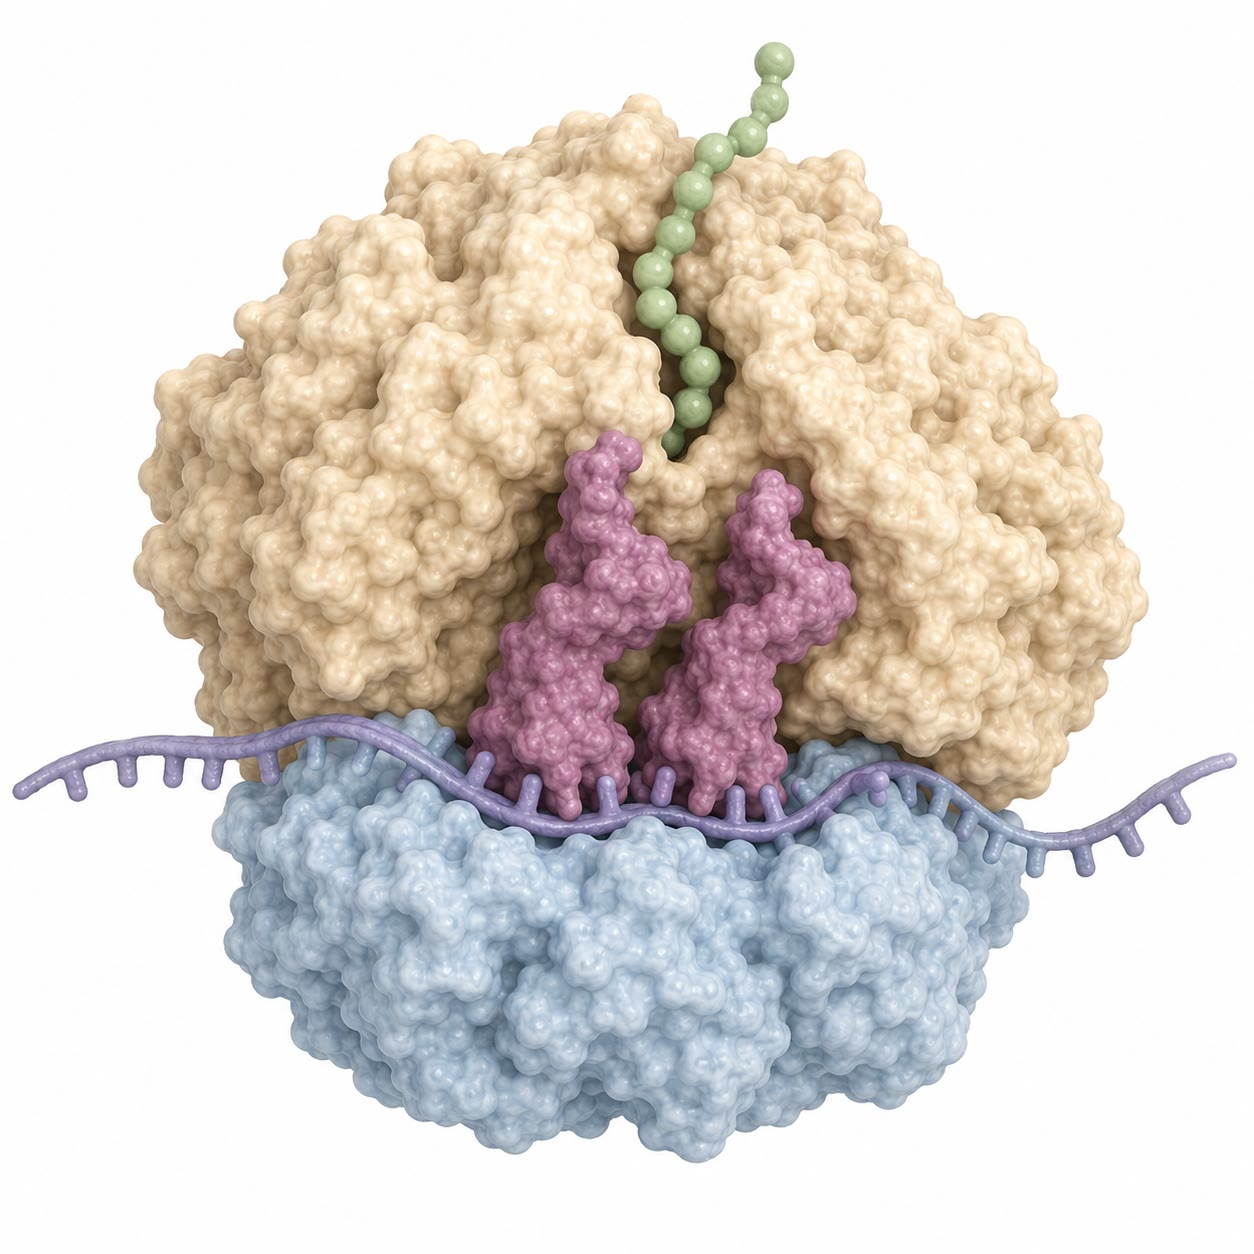
\includegraphics[width=0.46\linewidth]{images/book3/ai/fig-ribosome-3d.jpg}};
  \begin{scope}[x={(img.south east)}, y={(img.north west)},
      every node/.style={font=\small}]
    \draw[omDef, thick] (0.30,0.72) -- (0.30,1.08) node[above] {大亚基：在此形成肽键};
    \draw[omDef, thick] (0.50,0.15) -- (0.50,-0.08) node[below] {小亚基：解读信息};
    \draw[omDef, thick] (0.47,0.52) -- (-0.03,0.44) node[left, align=right] {位于 P 和 A 位点的 \\ 转运 RNA};
    \draw[omDef, thick] (0.92,0.36) -- (1.03,0.26) node[right] {信使 RNA};
    \draw[omDef, thick] (0.57,0.88) -- (1.03,0.90) node[right, align=left] {多肽经出口通道 \\ 离开};
  \end{scope}
\end{tikzpicture}

{\small \omterm{def:b1:gene-expression:ribosome}{核糖体}：两个亚基夹持信使 \omterm{def:b1:nucleic-acids:chain}{RNA}，两个
转运 \omterm{def:b1:nucleic-acids:chain}{RNA} 位于裂隙中，生长中的肽链经由
大亚基中的通道离开。}
\end{omfigure}

\begin{proposition}[延伸循环]\label{prop:b1:gene-expression:elongation}
翻译始于小亚基找到起始\omterm{def:b1:gene-expression:code}{密码子}——
在细菌中，靠\omterm{def:b1:gene-expression:ribosome}{核糖体} \omterm{def:b1:nucleic-acids:chain}{RNA} 的一段序列与紧邻
AUG 上游的位点配对；在真核生物中则是结合帽结构并扫描至
第一个 AUG——起始转运 \omterm{def:b1:nucleic-acids:chain}{RNA}（甲硫氨酸）落入 P
位点；随后大亚基结合。每一轮\emph{延伸}
增加一个残基：负载\omterm{def:b1:proteins:aminoacid}{氨基酸}的转运 \omterm{def:b1:nucleic-acids:chain}{RNA}，其\omterm{def:b1:gene-expression:trna}{反密码子}与 A 位点
上的\omterm{def:b1:gene-expression:code}{密码子}配对，经延伸因子送入并检验（消耗一个 GTP）；
大亚基的\omterm{def:b1:gene-expression:ribosome}{核糖体} \omterm{def:b1:nucleic-acids:chain}{RNA} 把生长中的肽链从
P 位点的转运 \omterm{def:b1:nucleic-acids:chain}{RNA} 转移到 A 位点转运 \omterm{def:b1:nucleic-acids:chain}{RNA} 的\omterm{def:b1:proteins:aminoacid}{氨基酸}上，形成
\omterm{def:b1:proteins:peptide}{肽键}；\omterm{def:b1:gene-expression:ribosome}{核糖体}前进一个\omterm{def:b1:gene-expression:code}{密码子}（消耗第二个 GTP），
使转运 \omterm{def:b1:nucleic-acids:chain}{RNA} 移至 P 和 E 位点，空载者离开。遇到终止
\omterm{def:b1:gene-expression:code}{密码子}时，\emph{释放因子}进入 A 位点，肽链被
水解释放。细菌\omterm{def:b1:gene-expression:ribosome}{核糖体}每秒添加 15 至 20 个残基，
真核\omterm{def:b1:gene-expression:ribosome}{核糖体}则为 2 至 5 个；多个\omterm{def:b1:gene-expression:ribosome}{核糖体}同时读取一条
信使，形成\emph{多聚\omterm{def:b1:gene-expression:ribosome}{核糖体}}。
\end{proposition}

\begin{omfigure}
\begin{tikzpicture}[font=\footnotesize, >=Stealth, line cap=round,
  rib/.style={draw, thick, rounded corners=8pt, fill=omDef!12, minimum width=30mm, minimum height=14mm},
  trna/.style={draw, thick, fill=omProp!30, minimum width=6mm, minimum height=9mm, inner sep=1pt, font=\scriptsize}]
  \foreach \i/\title in {0/{1. 携带氨基酸的 tRNA 进入 A 位}, 1/{2. 形成肽键：肽链转移到 A 位的 tRNA 上}, 2/{3. 移位：核糖体前移一个密码子}} {
    \begin{scope}[xshift=\i*4.5cm]
      \node[rib] (r) at (0,0) {};
      \draw[very thick, omThm] (-2.0,-0.9) -- (2.0,-0.9);
      \node[font=\scriptsize] at (-0.45,-0.55) {P}; \node[font=\scriptsize] at (0.45,-0.55) {A};
      \node[anchor=north, align=center, font=\scriptsize, text width=40mm] at (0,-1.75) {\title};
    \end{scope}
  }
  % state 1: P holds chain, A receives new tRNA
  \node[trna] at (-0.45,0.05) {}; \draw[very thick, omExo!70!black] (-0.45,0.5) -- (-0.45,1.4); \foreach \y in {0.6,0.85,1.1,1.35} { \fill[omExo!70!black] (-0.45,\y) circle (0.09); }
  \node[trna] at (0.45,0.05) {}; \fill[omExo!70!black] (0.45,0.6) circle (0.09);
  \draw[->, thick, omProp!80!black] (1.6,1.3) -- (0.75,0.7); \node[font=\scriptsize, anchor=west] at (1.4,1.45) {GTP};
  % state 2: chain transferred
  \node[trna] at (4.05,0.05) {}; \node[trna] at (4.95,0.05) {}; \draw[very thick, omExo!70!black] (4.95,0.5) -- (4.95,1.65); \foreach \y in {0.6,0.85,1.1,1.35,1.6} { \fill[omExo!70!black] (4.95,\y) circle (0.09); }
  % state 3: translocated: chain on P, empty tRNA leaving at E, A free
  \node[trna, fill=gray!20] at (7.6,0.05) {}; \node[trna] at (8.55,0.05) {}; \draw[very thick, omExo!70!black] (8.55,0.5) -- (8.55,1.65); \foreach \y in {0.6,0.85,1.1,1.35,1.6} { \fill[omExo!70!black] (8.55,\y) circle (0.09); }
  \draw[->, thick, gray] (7.6,-0.4) -- (7.0,-1.0); \node[font=\scriptsize, gray, anchor=east] at (7.05,-0.4) {E};
  \draw[->, thick, omProp!80!black] (10.7,0.3) -- (10.7,-0.3); \node[font=\scriptsize, anchor=west] at (10.8,0.3) {GTP};
    \draw[->, thick, omThm] (9.4,-1.3) -- (10.4,-1.3) node[right, font=\scriptsize, omThm] {mRNA 移动};
\end{tikzpicture}

{\small 一轮延伸。负载\omterm{def:b1:proteins:aminoacid}{氨基酸}的转运 \omterm{def:b1:nucleic-acids:chain}{RNA} 在
\omterm{def:b1:gene-expression:trna}{反密码子}匹配时进入 A 位点；\omterm{def:b1:gene-expression:ribosome}{核糖体} \omterm{def:b1:nucleic-acids:chain}{RNA} 将肽链
与其\omterm{def:b1:proteins:aminoacid}{氨基酸}相连，\omterm{def:b1:gene-expression:ribosome}{核糖体}前移一个\omterm{def:b1:gene-expression:code}{密码子}，空载的
转运 \omterm{def:b1:nucleic-acids:chain}{RNA} 离开。每个残基消耗两个 GTP，另加装载
转运 \omterm{def:b1:nucleic-acids:chain}{RNA} 时消耗的两个高能键。}
\end{omfigure}

\begin{omfigure}
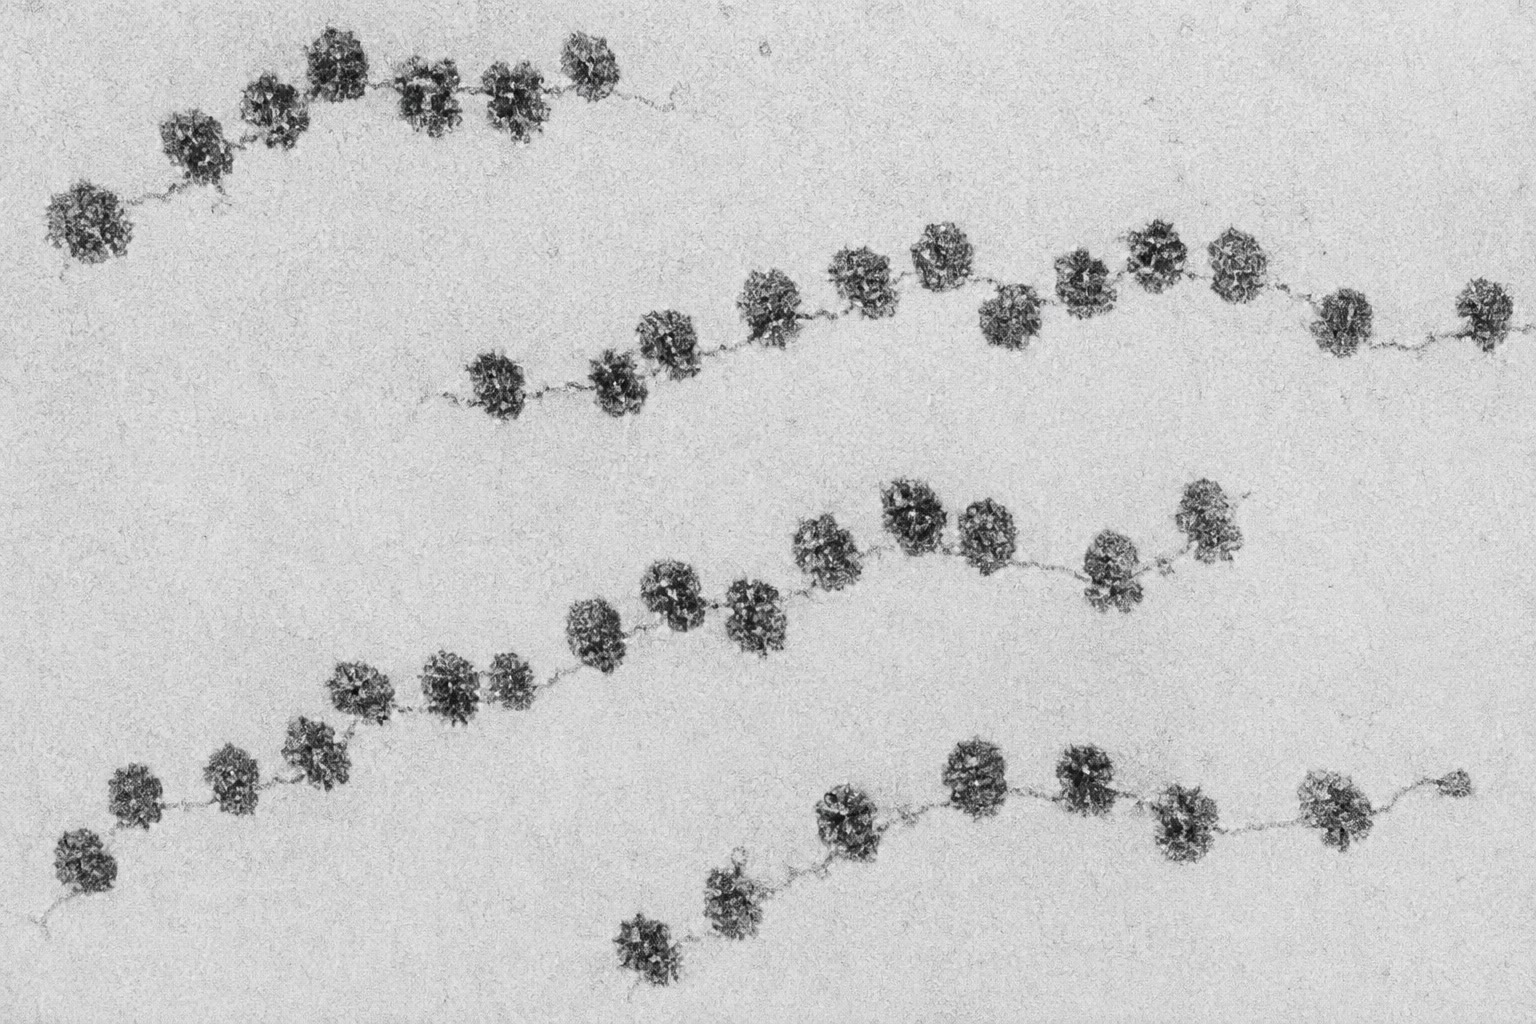
\includegraphics[width=0.5\linewidth]{images/book3/ai/b3-19-polysome-tem.jpg}

{\small \omterm{prop:b1:cell-unit-of-life:microscopes}{电子显微镜}下的多聚\omterm{def:b1:gene-expression:ribosome}{核糖体}：多个\omterm{def:b1:gene-expression:ribosome}{核糖体}沿
同一条信使串联排列，各自合成一份该\omterm{def:b1:proteins:peptide}{蛋白质}。}
\end{omfigure}

\begin{method}[估算蛋白质合成]\label{met:b1:gene-expression:reckon}
\begin{enumerate}
  \item 长度：含 $n$ 个残基的\omterm{def:b1:proteins:peptide}{蛋白质}，其编码序列需为
        $3n + 3$ 个\omterm{def:b1:nucleic-acids:nucleotide}{核苷酸}（含终止\omterm{def:b1:gene-expression:code}{密码子}），位于一条
        更长的信使中，比编码序列多出其非翻译末端；在\omterm{def:b1:genomes:gene}{基因}中，
        还要再加上\omterm{def:b1:genomes:gene}{内含子}。
  \item 时间：用 $n$ 除以延伸速率（细菌中为 \qtyrange{15}{20}{}
        每秒，真核生物中为 \qtyrange{2}{5}{}）；
        信使上每隔 \qtyrange{80}{100}{} 个\omterm{def:b1:nucleic-acids:nucleotide}{核苷酸}便有
        一个\omterm{def:b1:gene-expression:ribosome}{核糖体}在读取，故每条信使的产出为每隔
        （间距 / 速率）秒一条肽链。
  \item 能量：每个残基消耗四个高能磷酸键（两个用于
        装载转运 \omterm{def:b1:nucleic-acids:chain}{RNA}，两个 GTP 在\omterm{def:b1:gene-expression:ribosome}{核糖体}上），另加
        信使转录（每个\omterm{def:b1:nucleic-acids:nucleotide}{核苷酸}两个），由该
        信使产生的所有肽链共同分摊。
  \item 保真度：每 $10^4$ 个\omterm{def:b1:gene-expression:code}{密码子}中约有一个错误\omterm{def:b1:proteins:aminoacid}{氨基酸}；含
        \qty{500}{} 个残基的\omterm{def:b1:proteins:peptide}{蛋白质}，约在二十分之一的拷贝中
        某处出错——可以容忍，因为\omterm{def:b1:proteins:peptide}{蛋白质}可以替换，
        且错误不会遗传。
\end{enumerate}
\end{method}

\section{翻译之后}

\begin{proposition}[新生多肽的去向]\label{prop:b1:gene-expression:after}
\index{信号肽}\index{翻译后修饰}
肽链在伸出时即开始折叠，并借助\omterm{prop:b1:proteins:denaturation}{分子伴侣}
（\cref{ch:b1:proteins}）。其去向写在其序列中：
位于 N 端的\emph{\omterm{prop:b1:gene-expression:after}{信号肽}}与\emph{信号
\omterm{prop:b1:water-small-molecules:weak}{识别}颗粒}结合，使翻译暂停，并使\omterm{def:b1:gene-expression:ribosome}{核糖体}对接到
\omterm{def:b1:eukaryotic-cell:endomembrane}{内质网}上，并将肽链穿入其腔中
（\cref{ch:b1:eukaryotic-cell}）；其他序列则将\omterm{def:b1:proteins:peptide}{蛋白质}导入
\omterm{def:b1:eukaryotic-cell:mitochondrion}{线粒体}、\omterm{def:b1:photosynthesis:chloroplast}{叶绿体}、\omterm{def:b1:eukaryotic-cell:nucleus}{细胞核}或\omterm{def:b1:eukaryotic-cell:peroxisome}{过氧化物酶体}，均在合成之后进行；
无信号的\omterm{def:b1:proteins:peptide}{蛋白质}则留在\omterm{def:b1:eukaryotic-cell:organelle}{细胞溶胶}中。许多
\omterm{def:b1:proteins:peptide}{蛋白质}会被\emph{修饰}：去除起始的甲硫氨酸，
在\omterm{def:b1:eukaryotic-cell:endomembrane}{内质网}和\omterm{def:b1:eukaryotic-cell:endomembrane}{高尔基体}中连接\omterm{def:b1:carbohydrates:monosaccharide}{糖类}，由激酶添加、由磷酸酶去除磷酸基团，
连接脂质，切除部分片段（胰岛素先合成一条链，
再切为两段；酶原经切割而被激活）。此外，
每种\omterm{def:b1:proteins:peptide}{蛋白质}最终都会被\emph{降解}：先被小蛋白
\emph{泛素}标记，再由
\emph{蛋白酶体}展开并消化，其寿命从几分钟（调节蛋白）
到几个月（血红蛋白）不等——因此\omterm{def:b1:cell-unit-of-life:cell}{细胞}中现存的\omterm{def:b1:proteins:peptide}{蛋白质}
恰是\omterm{def:b1:cell-unit-of-life:cell}{细胞}当前正在合成的那些。
\end{proposition}

\begin{example}[细胞中的数量]\label{ex:b1:gene-expression:numbers}
处于生长期的\emph{E. coli}含有约 \num{20000} 个\omterm{def:b1:gene-expression:ribosome}{核糖体}，每个\omterm{def:b1:gene-expression:ribosome}{核糖体}
每秒加入二十个残基，合计每秒 $\num{4e5}$ 个残基，
即每小时合成一百万个含 \qty{300}{} 个残基的\omterm{def:b1:proteins:peptide}{蛋白质}——恰为其自身的
全部内容，正是每小时倍增所需的量。其能量的一半
用于\omterm{def:b1:proteins:peptide}{蛋白质}合成。肝\omterm{def:b1:cell-unit-of-life:cell}{细胞}含一千万个\omterm{def:b1:gene-expression:ribosome}{核糖体}，
却合成可供数周使用的\omterm{def:b1:proteins:peptide}{蛋白质}，而不用于分裂；
浆\omterm{def:b1:cell-unit-of-life:cell}{细胞}分泌抗体，几乎把全部\omterm{def:b1:gene-expression:ribosome}{核糖体}用于
合成同一种\omterm{def:b1:proteins:peptide}{蛋白质}，每秒产出两千个分子。
\end{example}

\section{练习}

\begin{exercise}[$\star$]\label{exo:b1:gene-expression:1}
写出由模板链
$3'$-TACGGATTC-$5'$ 转录得到的 \omterm{def:b1:nucleic-acids:chain}{RNA}，并写出编码链。
\end{exercise}

\begin{exercise}[$\star$]\label{exo:b1:gene-expression:2}
列出真核生物初级转录本
离开\omterm{def:b1:eukaryotic-cell:nucleus}{细胞核}之前所经历的三种修饰。
\end{exercise}

\begin{exercise}[$\star$]\label{exo:b1:gene-expression:3}
依据\omterm{def:b1:gene-expression:code}{遗传密码}表，翻译 $5'$-AUGCCGAAAGUUUGA-$3'$。
\end{exercise}

\begin{exercise}[$\star$]\label{exo:b1:gene-expression:4}
写出\omterm{def:b1:gene-expression:ribosome}{核糖体}上的三个 tRNA 位点，并说明每个位点上发生的过程。
\end{exercise}

\begin{exercise}[$\star\star$]\label{exo:b1:gene-expression:5}
一条长 \qty{2400}{} 个\omterm{def:b1:nucleic-acids:nucleotide}{核苷酸}的信使 \omterm{def:b1:nucleic-acids:chain}{RNA}，其 $5'$
非翻译区长 \qty{150}{}，$3'$ 非翻译区长 \qty{450}{}，并带有
poly-A 尾。该\omterm{def:b1:proteins:peptide}{蛋白质}含多少个残基？一个\omterm{def:b1:gene-expression:ribosome}{核糖体}以每秒四个残基的速度
需要多长时间才能合成完毕？若每 \qty{90}{} 个\omterm{def:b1:nucleic-acids:nucleotide}{核苷酸}
只容纳一个\omterm{def:b1:gene-expression:ribosome}{核糖体}，则同一时刻能有多少个\omterm{def:b1:gene-expression:ribosome}{核糖体}读取该信使？
\end{exercise}

\begin{exercise}[$\star\star$]\label{exo:b1:gene-expression:6}
解释为什么三次插入能恢复\omterm{def:b1:genomes:gene}{基因}的\omterm{def:b1:gene-expression:code}{阅读框}，而一次
或两次插入则不能，并说明由三次插入产生的\omterm{def:b1:proteins:peptide}{蛋白质}
是什么样子。
\end{exercise}

\begin{exercise}[$\star\star$]\label{exo:b1:gene-expression:7}
在一个含 \qty{300}{} 个\omterm{def:b1:gene-expression:code}{密码子}的\omterm{def:b1:genomes:gene}{基因}中部，某突变使\omterm{def:b1:gene-expression:code}{密码子} CAG
变为 UAG；另一突变使 CAG 变为 CAA，第三种突变则使其变为
CGG。试分别说明每种突变对\omterm{def:b1:proteins:peptide}{蛋白质}的影响。
\end{exercise}

\begin{exercise}[$\star\star$]\label{exo:b1:gene-expression:8}
解释翻译的保真度为何取决于氨酰 tRNA 合成酶，
而非\omterm{def:b1:gene-expression:ribosome}{核糖体}，并描述一项能证明这一点的实验
（将连接在其 tRNA 上的半胱氨酸经化学转变为
丙氨酸；丙氨酸最终会出现在何处？）。
\end{exercise}

\begin{exercise}[$\star\star$]\label{exo:b1:gene-expression:9}
计算一个含 \qty{400}{} 个残基的\omterm{def:b1:proteins:peptide}{蛋白质}的能量成本，
以高能磷酸键计，并求其中耗在\omterm{def:b1:gene-expression:ribosome}{核糖体}上的比例。
\end{exercise}

\begin{exercise}[$\star\star\star$]\label{exo:b1:gene-expression:10}
在细菌中，\omterm{def:b1:gene-expression:ribosome}{核糖体}在信使 \omterm{def:b1:nucleic-acids:chain}{RNA} 仍在被转录时即开始翻译，
而在真核生物中则不能。试解释原因（两点），
并说明这一差异使真核生物能够实现何种过程。
\end{exercise}

\begin{exercise}[$\star\star\star$]\label{exo:b1:gene-expression:11}
一个含五个\omterm{def:b1:genomes:gene}{外显子}的\omterm{def:b1:genomes:gene}{基因}，其剪接可以保留或跳过\omterm{def:b1:genomes:gene}{外显子} 3
（\qty{90}{} 个\omterm{def:b1:nucleic-acids:nucleotide}{核苷酸}）和\omterm{def:b1:genomes:gene}{外显子} 4（\qty{100}{} 个\omterm{def:b1:nucleic-acids:nucleotide}{核苷酸}）。列出
所有可能的信使 \omterm{def:b1:nucleic-acids:chain}{RNA}，并指出其中哪些能保持
\omterm{def:b1:genomes:gene}{外显子} 5 的\omterm{def:b1:gene-expression:code}{阅读框}。这说明了可变剪接的什么问题？
\end{exercise}

\begin{exercise}[$\star\star\star$]\label{exo:b1:gene-expression:12}
“\omterm{def:b1:gene-expression:code}{遗传密码}是一场冻结的偶然：任意，但改变的代价过于高昂。”
试用一段文字讨论：\omterm{def:b1:gene-expression:code}{遗传密码}中哪些看似任意，哪些
看似经过优化（第三位碱基，以及相似\omterm{def:b1:proteins:aminoacid}{氨基酸}对应
相似\omterm{def:b1:gene-expression:code}{密码子}），并说明为何改变某一合成酶专一性的突变
几乎总是致死的。
\end{exercise}

\section{问题：从基因到蛋白质}

\begin{problem}[{周末问题——追踪一个三十千碱基的基因，
得到一条五百残基的蛋白质：计时转录，称量剪接，
计数核糖体，核算能量与误差，最后落在一个
蛋白质以 ATP 计的成本上}]
\label{pb:b1:gene-expression:1}
一个人类\omterm{def:b1:genomes:gene}{基因}跨度为 \qty{30}{kb}，含八个\omterm{def:b1:genomes:gene}{外显子}，
其成熟信使 \omterm{def:b1:nucleic-acids:chain}{RNA} 共 \qty{2000}{} 个\omterm{def:b1:nucleic-acids:nucleotide}{核苷酸}，其中 \qty{1503}{} 个
\omterm{def:b1:nucleic-acids:nucleotide}{核苷酸}用于编码（500 个残基加一个终止\omterm{def:b1:gene-expression:code}{密码子}）。\omterm{def:b1:nucleic-acids:chain}{RNA} 聚合酶 II 以
每秒 \qty{30}{} 个\omterm{def:b1:nucleic-acids:nucleotide}{核苷酸}的速度转录；\omterm{def:b1:gene-expression:ribosome}{核糖体}的延伸速率为每秒
\qty{4}{} 个残基，并沿信使每 \qty{80}{} 个\omterm{def:b1:nucleic-acids:nucleotide}{核苷酸}排列一个；
信使 \omterm{def:b1:nucleic-acids:chain}{RNA} 的半衰期为 \qty{2}{h}。成本如下：每转录一个\omterm{def:b1:nucleic-acids:nucleotide}{核苷酸}消耗
两个高能键，每翻译一个残基消耗四个。
取一个高能键为一个 \omterm{def:b1:water-small-molecules:atp}{ATP}。错误率为：
每个转录的\omterm{def:b1:nucleic-acids:nucleotide}{核苷酸} $10^{-5}$，每个翻译的\omterm{def:b1:gene-expression:code}{密码子} $10^{-4}$。

\medskip
\noindent\textbf{第一部分——转录与剪接。}
\begin{enumerate}
  \item 一个聚合酶转录该\omterm{def:b1:genomes:gene}{基因}需要多长时间？
  \item 剪接去除的
        初级转录本占多大比例？
  \item 为得到每个成熟信使的\omterm{def:b1:nucleic-acids:nucleotide}{核苷酸}，
        需转录多少个\omterm{def:b1:nucleic-acids:nucleotide}{核苷酸}？
  \item 计算转录一个初级转录本所消耗的 \omterm{def:b1:water-small-molecules:atp}{ATP}。
  \item 若每隔 \qty{10}{s} 起始一个聚合酶，
        \omterm{def:b1:genomes:gene}{基因}上同时有多少个聚合酶，
        该\omterm{def:b1:genomes:gene}{基因}每小时产生多少个信使？
  \item 计算\omterm{def:b1:genomes:gene}{内含子}的数目及其平均长度。
  \item 剪接体在约一分钟内
        并行去除每个\omterm{def:b1:genomes:gene}{内含子}。决定
        从\omterm{def:b1:genomes:gene}{基因}到信使所需时间的是剪接还是转录？
  \item 计算\omterm{def:b1:genomes:gene}{基因}和成熟信使的物理长度
        （每个\omterm{def:b1:nucleic-acids:nucleotide}{核苷酸}为 \qty{0.34}{nm}）。
\end{enumerate}

\medskip
\noindent\textbf{第二部分——翻译。}
\begin{enumerate}[resume]
  \item 一个\omterm{def:b1:gene-expression:ribosome}{核糖体}翻译该\omterm{def:b1:proteins:peptide}{蛋白质}需要多长时间？
  \item 同时有多少个\omterm{def:b1:gene-expression:ribosome}{核糖体}在读取同一条信使？
  \item 每条信使每
        小时产生多少个\omterm{def:b1:proteins:peptide}{蛋白质}分子？
  \item 在其 \qty{2}{h} 的半衰期内，共产生多少个\omterm{def:b1:proteins:peptide}{蛋白质}分子
        （半衰期为 $t_{1/2}$ 的信使平均可
        满负荷生产 $t_{1/2}/\ln 2$ 小时）？
  \item 计算翻译一个\omterm{def:b1:proteins:peptide}{蛋白质}所消耗的 \omterm{def:b1:water-small-molecules:atp}{ATP}。
  \item 计算每个\omterm{def:b1:proteins:peptide}{蛋白质}分摊的转录成本，
        即将转录本的成本在第 12 题所涉及的\omterm{def:b1:proteins:peptide}{蛋白质}之间分摊。
  \item 计算一个\omterm{def:b1:proteins:peptide}{蛋白质}的总成本，以及
        翻译所占的比例。
\end{enumerate}

\medskip
\noindent\textbf{第三部分——错误。}
\begin{enumerate}[resume]
  \item 计算某条给定信使的
        \qty{1503}{} 个编码\omterm{def:b1:nucleic-acids:nucleotide}{核苷酸}中至少含一个
        转录错误的概率。
  \item 计算某个给定\omterm{def:b1:proteins:peptide}{蛋白质}分子
        中至少含一个翻译错误的概率。
  \item 约四分之一的\omterm{def:b1:nucleic-acids:nucleotide}{核苷酸}改变是沉默的，
        三分之一的\omterm{def:b1:proteins:aminoacid}{氨基酸}替换是无害的。
        所产生的\omterm{def:b1:proteins:peptide}{蛋白质}分子中有多大比例是有缺陷的？
  \item 一条有缺陷的信使在两小时内产生有缺陷的\omterm{def:b1:proteins:peptide}{蛋白质}，
        而每个有缺陷的\omterm{def:b1:proteins:peptide}{蛋白质}是一个分子。解释\omterm{def:b1:cell-unit-of-life:cell}{细胞}为何能够承受
        比转录错误率高十倍的翻译错误率，
        而这两者都远高于复制错误率。
\end{enumerate}

\medskip
\noindent\textbf{第四部分——\omterm{def:b1:cell-unit-of-life:cell}{细胞}的预算。}
\omterm{def:b1:cell-unit-of-life:cell}{细胞}每小时制造 \num{3000} 个该\omterm{def:b1:proteins:peptide}{蛋白质}分子，
        每天共制造 \num{3e9} 个残基的\omterm{def:b1:proteins:peptide}{蛋白质}。
\begin{enumerate}[resume]
  \item 该\omterm{def:b1:genomes:gene}{基因}的信使必须同时存在多少个
        （每个信使的产量见第 11 题）？
  \item 有多少个\omterm{def:b1:gene-expression:ribosome}{核糖体}被该\omterm{def:b1:proteins:peptide}{蛋白质}占用？
  \item 计算\omterm{def:b1:cell-unit-of-life:cell}{细胞}每天用于全部\omterm{def:b1:proteins:peptide}{蛋白质}合成的 \omterm{def:b1:water-small-molecules:atp}{ATP}
        （每个残基四个），并在 \qty{50}{kJ/mol} 下，
        计算体积为 \qty{2000}{\micro m^3} 的\omterm{def:b1:cell-unit-of-life:cell}{细胞}的功率（瓦特）。
  \item 将其与\omterm{def:b1:cell-unit-of-life:cell}{细胞}每秒消耗
        \qty{1e9}{} 个 \omterm{def:b1:water-small-molecules:atp}{ATP} 时的总功率相比较。
  \item 一种药物阻断剪接体。预测其对该\omterm{def:b1:proteins:peptide}{蛋白质}
        及一种细菌\omterm{def:b1:proteins:peptide}{蛋白质}的影响。
  \item 给出结果：一个\omterm{def:b1:proteins:peptide}{蛋白质}分子的 \omterm{def:b1:water-small-molecules:atp}{ATP} 成本
        （在翻译与转录之间划分），以及从转录开始
        到第一个完成的\omterm{def:b1:proteins:peptide}{蛋白质}所需的
        时间。
\end{enumerate}
\end{problem}
